% this TeX file provides an awesome example of how TeX will make super 
% awesome tables, at the cost of your of what happens when you try to make a
% table that is very complicated.
% Originally turned in for Dr. Nico's Security Class
\documentclass[11pt]{article}
\usepackage[a4,margin=1in]{geometry}


\usepackage[utf8]{inputenc}
\usepackage{graphicx}
\usepackage{tikz}
\def\checkmark{\tikz\fill[scale=0.4](0,.35) -- (.25,0) -- (1,.7) -- (.25,.15) -- cycle;} 

% multirow allows you to combine rows in columns
\usepackage{multirow}
% tabularx allows manual tweaking of column width
\usepackage{tabularx}
% longtable does better format for tables that span pages
\usepackage{longtable}

\begin{document}
\setlength{\parindent}{0pt}
% this is an alternate method of creating a title
%\hfill\vbox{\hbox{Gius, Mark}
%       \hbox{Cpe 456, Section 01}  
%       \hbox{Lab 1}    
%       \hbox{\today}}\par
%
%\bigskip
%\centerline{\Large\bf Lab 1: Security Audit}\par
%\bigskip
\author{Grégoire Hirt\\ Marc Bickel\\ Raphaël Barman}
\title{\vspace{-2.0cm}Report: Part 1}
\maketitle
\vspace{-1cm}
\section{State of the project}
Since an image is better than a thousand words, here is one:
\begin{center}
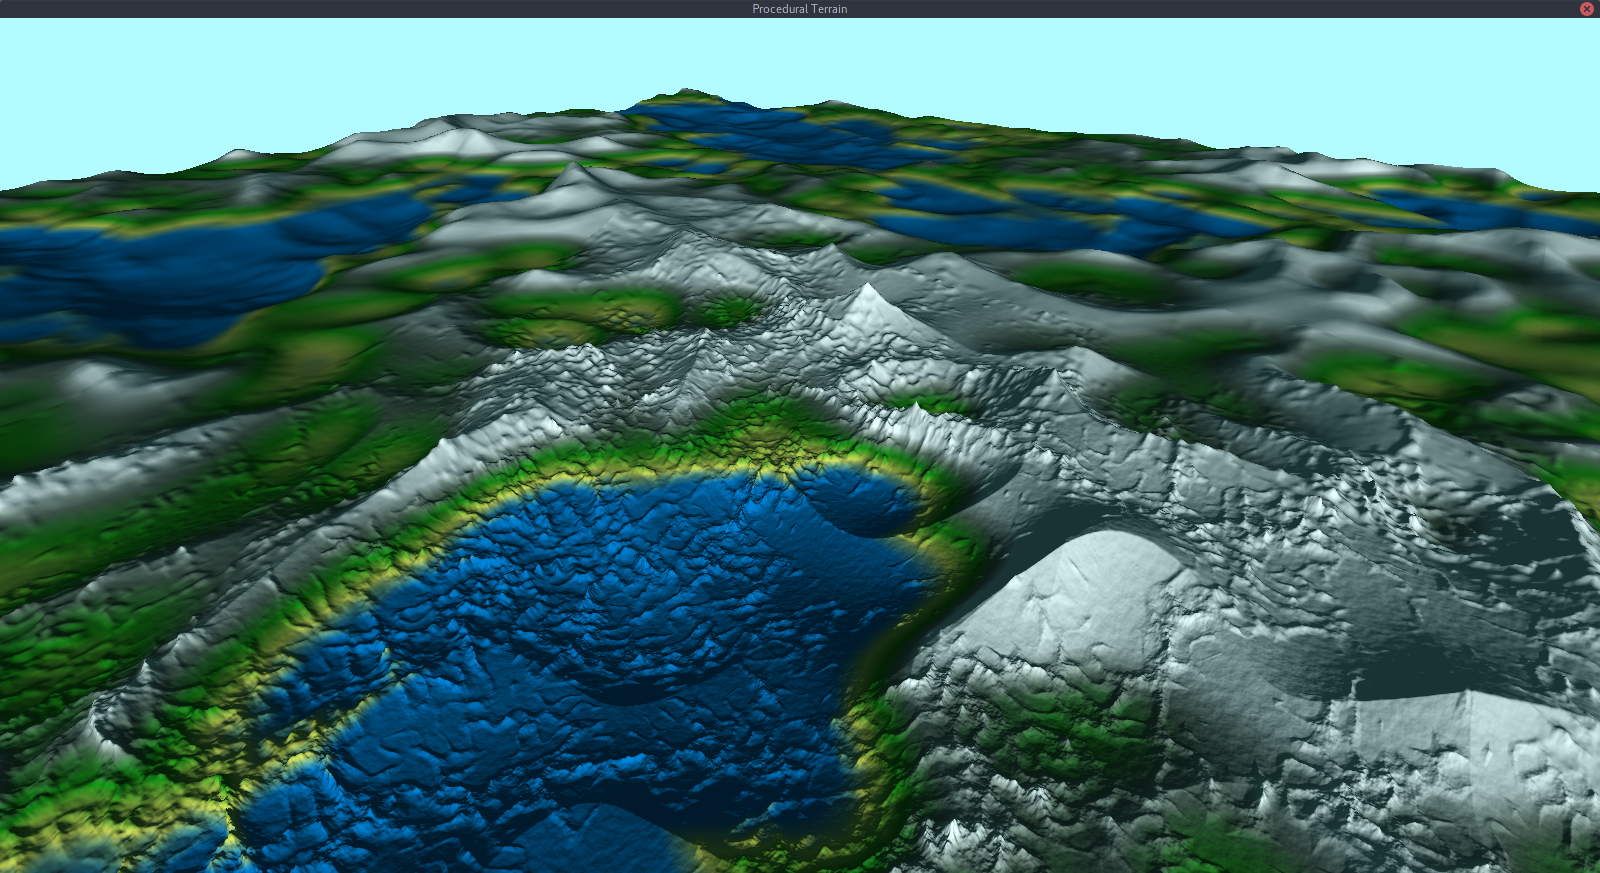
\includegraphics[width=\textwidth]{screen03}
\caption{Current state of the project}
\end{center} \\

What we implemented during this first part was:
\begin{itemize}
\item Height map generation from a noise
\item Perlin Noise
\item Simplex Noise
\item Fractal Brownian motion
\item Ridged hybrid multifractal
\item Grid with height defined by an heightmap
\item Phong shading
\item Coloring according to height map
\item Chunk system for infinite terrain
\end{itemize}
The height map texture is created on a framebuffer using the noise and fbm/rhm and passed to the grid, which
uses it to change its height.

The normal we used in Phong shading is computed using finite methods.

The coloring is done using the height and a 1D color texture as done in the
previous labs.\\

\begin{center}
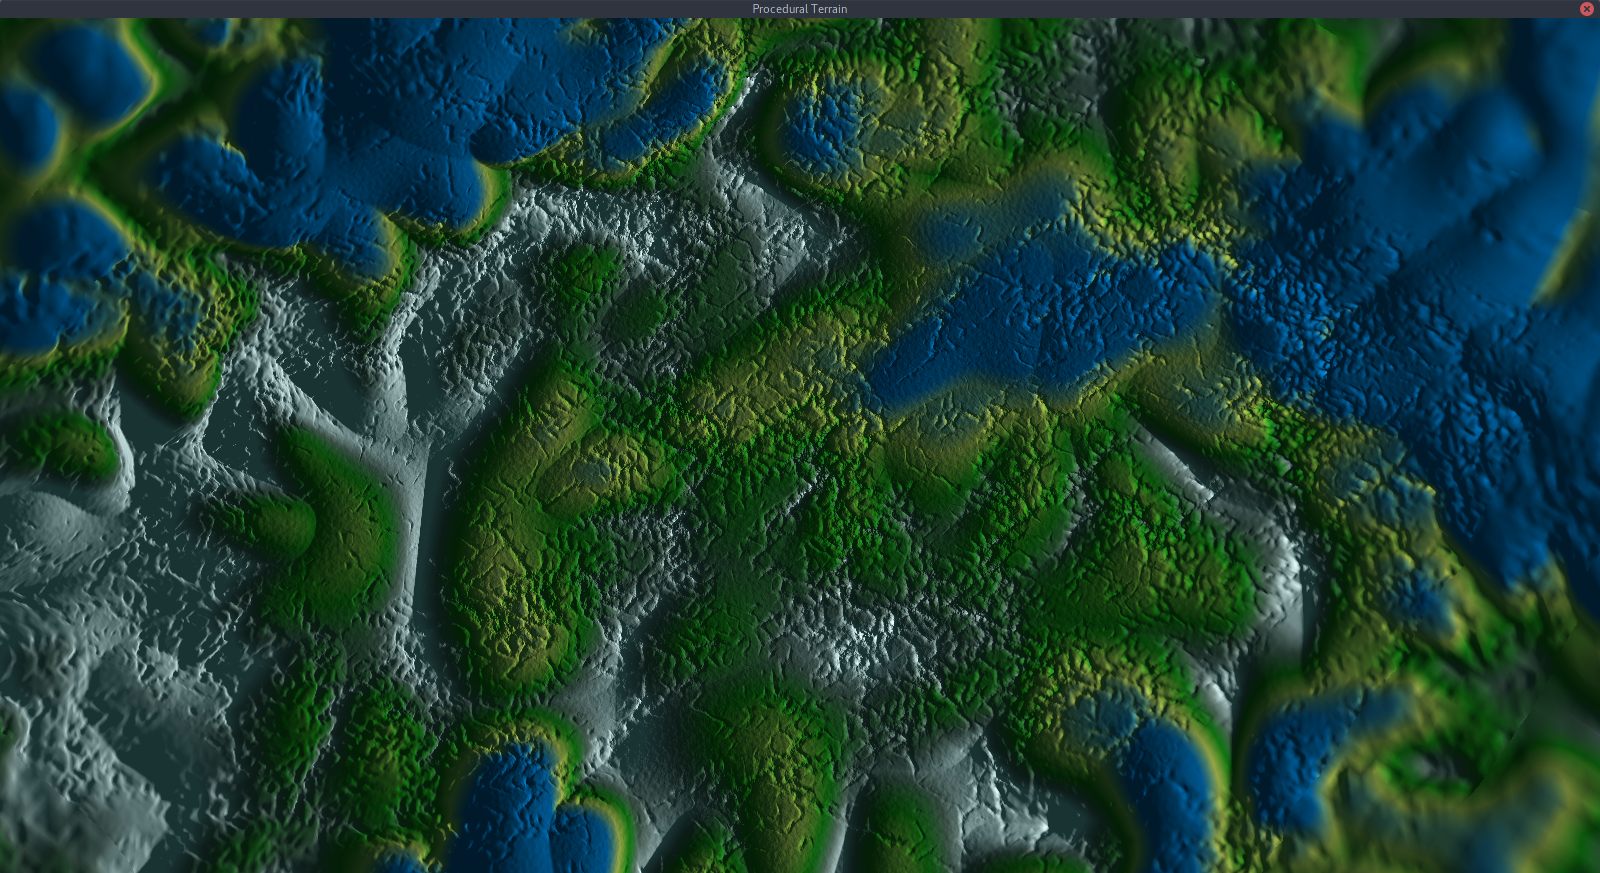
\includegraphics[width=\textwidth]{screen02}
\caption{Top view}
\end{center} \\

We will now present some more detailed information on the non-compulsory parts.

\subsection{Height map generation}
Since we decided to aim at maximum performance from the very beginning, we
choose to implement simplex noise algorithm. In the future we may need a higher
dimension than 2D for our noise (to counter the fact that when we go very far in
our infinite terrain, the noise becomes unstable because of floating point
rounding), the cost of simplex noise is $O(n^2)$ for $n$ dimension, whereas the
Perlin noise cost is of $O(2^n)$. Simplex noise mainly differs from Perlin in the fact that it is interpolating over equilateral triangles and not squares. The fact that it uses a circular kernel also add lumpiness to the image.

Our noise generation is then just a combination of multiple layer of this noise.
We currently use two ridged multi-fractal parts that also controls fbm amounts.
\subsection{Chunk system for infinite terrain}
One feature that we already implemented is a chunk-based lod-system. This is not using hardware tesselation but we instead manage a set of spacially indexed chunks that represents parts of the terrain. Theses chunks can be drawn at different resolution allowing to simplify drawing at large distances.

To avoid visual artifact at chunk edges we use skirts and the noise function is sampled with 1px margin so that we still can derivate normals at chunks edges.

The chunk updates are put into a worker queue that is then executed over multiple frame to prevent chunk switching to create stuttering. This chunk system is teleport-proof, meaning one can change camera position arbitrarily far and still generate and remove the right chunks.

In the future, we might switch to a quadtree-based chunk system and improve the noise texture cache.

\begin{center}
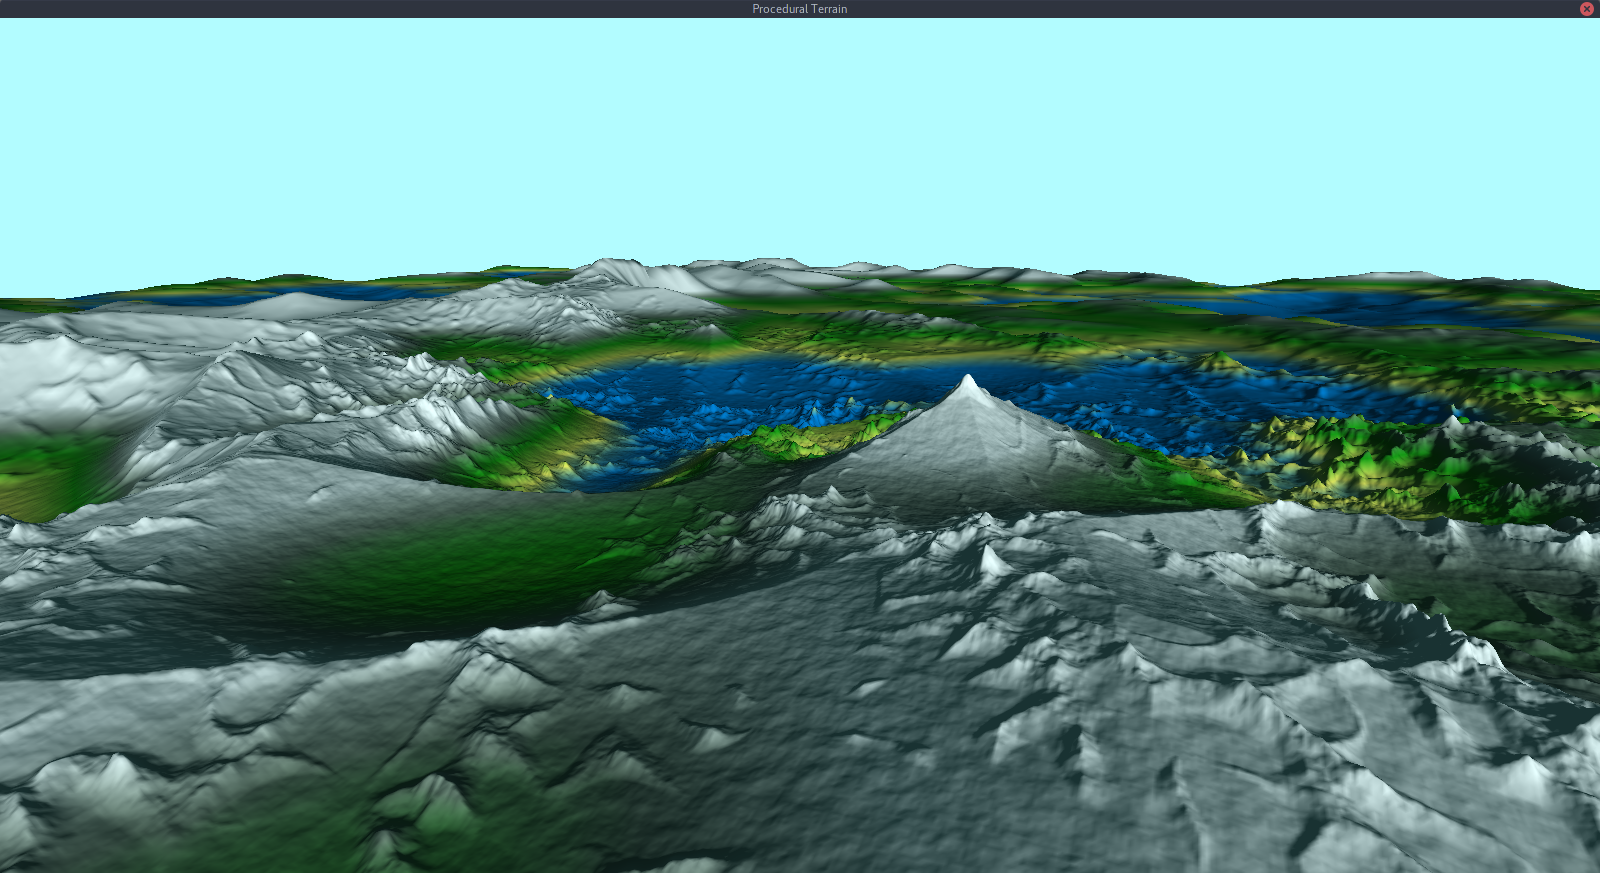
\includegraphics[width=\textwidth]{screen01}
\caption{Another view of the current state}
\end{center} \\

\section{Work distribution}
\subsection{Mandatory part}

\begin{tabular}{l|ccc}
 & Marc & Grégoire & Raphaël \\ \hline
Framebuffer from noise &   & \checkmark & \checkmark \\
Perlin noise &\checkmark  &\checkmark  &  \\
FBM &  & \checkmark &  \\
Phong & \checkmark &  &  \\
Grid with height & & & \checkmark\\ 
Coloring &  \checkmark &\checkmark  & \checkmark
\end{tabular}

\subsection{Extra part}

\begin{tabular}{l|ccc}
 & Marc & Grégoire & Raphaël \\ \hline
Simplex noise &  \checkmark & \checkmark &  \\
Ridged hybrid multifractal &&\checkmark  & \checkmark \\
Chunk system &  & \checkmark & 
\end{tabular}

\end{document}
